\subsection{Admission frequency through a later cutoff}\label{app:candidate-retained-trace}

\Cref{fig:fw-candidate-retained-trace} groups the complete admission journal
from the canonical ledger's first round (\cref{tab:admission-ledger}) through
the latest complete admission matched to a retained summary. Its 24 blocks
contain 23 full blocks and one partial block; 19 have no admission, including
17 consecutive full blocks in rounds 975--2674. The 21 available summaries
(3145--3165) match the journal's scores and decisions; older rows are journal-only.
The last accepted decision, at round 3100, is an exact tie, followed by
65 rejections. Frequencies count decisions, not independent tasks, distinct
programs or a stationary admission probability. Stable log-prefix hashes bind
this separate capture. This trace retains its own capture cutoff;
the field-binding limits in \cref{sec:method-status} still apply.

\begin{figure*}[!t]
  \setlength{\abovecaptionskip}{4pt}
  \centering
  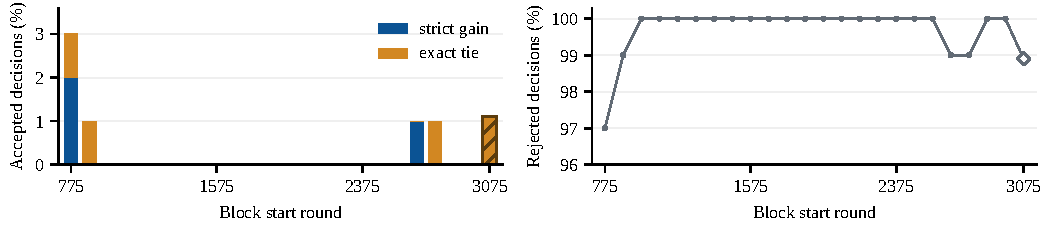
\includegraphics[width=\linewidth,height=1.55in,keepaspectratio]{figures/fig_fw_admission_block_rates.pdf}
  \caption{\textbf{Adapter admission and rejection frequencies by observed-round block.}
  All \num{2391} complete journal decisions in rounds 775--3165, captured at 20:17 UTC
  on 1 November 2026. Blocks contain 100 consecutive observed rounds; the final
  3075--3165 block contains 91. Left: accepted strict gains (blue) and exact ties
  (orange), stacked percentages. Right: rejected decisions (percent; axis starts
  at 96\%). Each denominator is that block's observed rounds; hatching and a
  diamond mark the partial block. Totals: 3 strict gains, 4 ties and
  \num{2384} rejections. These adaptive adapter decisions are distinct from
  program-incumbent events and independent first-proposal performance.
  Scope: \cref{sec:method-status}.}
  \label{fig:fw-candidate-retained-trace}
\end{figure*}
